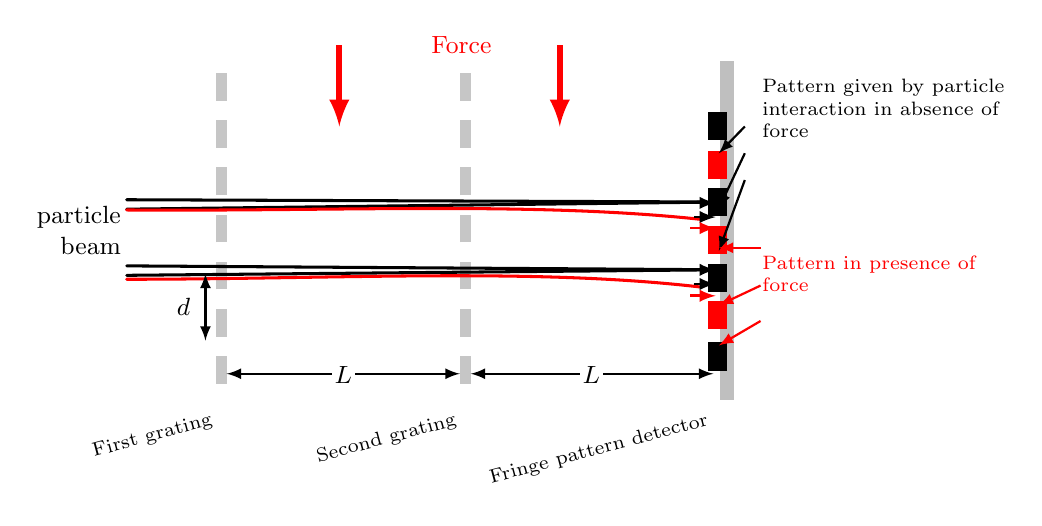
\begin{tikzpicture}[
  x=1cm,y=1cm,
  beam/.style={line width=1.1pt,line cap=round},
  force/.style={-latex,red,line width=2.3pt},
  label/.style={font=\small},
  smalllabel/.style={font=\scriptsize},
  dim/.style={latex-latex,line width=0.8pt},
  callout/.style={-latex,line width=0.8pt},
  redcallout/.style={-latex,red,line width=0.8pt}
]
  \def\gOne{1.25}
  \def\gTwo{4.35}
  \def\det{7.55}

  \foreach \x in {\gOne,\gTwo}{
    \foreach \y in {0.45,1.05,1.65,2.25,2.85,3.45,4.05}{
      \draw[gray!45,line width=4pt] (\x,\y) -- (\x,\y+0.35);
    }
  }

  \draw[gray!50,line width=5pt] (\det+0.12,0.25) -- (\det+0.12,4.55);
  \foreach \y/\c in {0.62/black,1.15/red,1.62/black,2.10/red,2.58/black,3.05/red,3.55/black}{
    \draw[\c,line width=7pt] (\det,\y) -- (\det,\y+0.36);
  }

  \node[label,align=right,anchor=east] at (0.10,2.40) {particle\\beam};
  \node[label,red] at (4.30,4.75) {Force};
  \draw[force] (2.75,4.75) -- (2.75,3.72);
  \draw[force] (5.55,4.75) -- (5.55,3.72);

  \foreach \dy in {-0.05,0.07}{
    \draw[beam,black] (0.05,2.72+\dy) -- (\det-0.20,2.76+0.03*\dy);
    \draw[beam,black] (0.05,1.88+\dy) -- (\det-0.20,1.90+0.03*\dy);
  }
  \draw[beam,red] (0.05,2.66) .. controls (2.7,2.64) and (5.2,2.77) .. (\det-0.20,2.54);
  \draw[beam,red] (0.05,1.78) .. controls (2.7,1.78) and (5.2,1.93) .. (\det-0.20,1.68);

  \foreach \y in {2.57,2.75,1.72,1.90}{
    \draw[-latex,line width=1pt] (\det-0.30,\y) -- (\det-0.02,\y);
  }
  \draw[-latex,red,line width=1pt] (\det-0.34,2.43) -- (\det-0.02,2.43);
  \draw[-latex,red,line width=1pt] (\det-0.34,1.57) -- (\det-0.02,1.57);

  \draw[dim] (\gOne-0.20,1.00) -- (\gOne-0.20,1.85);
  \node[label,fill=white,inner sep=1pt] at (\gOne-0.48,1.43) {$d$};

  \draw[dim] (\gOne+0.07,0.58) -- (\gTwo-0.07,0.58);
  \node[label,fill=white,inner sep=1pt] at ({(\gOne+\gTwo)/2},0.56) {$L$};
  \draw[dim] (\gTwo+0.07,0.58) -- (\det-0.05,0.58);
  \node[label,fill=white,inner sep=1pt] at ({(\gTwo+\det)/2},0.56) {$L$};

  \node[smalllabel,align=center,rotate=15,anchor=east] at (\gOne,0.02) {First grating};
  \node[smalllabel,align=center,rotate=15,anchor=east] at (\gTwo,0.02) {Second grating};
  \node[smalllabel,align=center,rotate=15,anchor=east] at (\det,0.02) {Fringe pattern detector};

  \node[smalllabel,align=left,anchor=west] (absent) at (8.00,3.95) {Pattern given by particle\\interaction in absence of\\force};
  \draw[callout] (7.90,3.72) -- (\det+0.02,3.38);
  \draw[callout] (7.90,3.38) -- (\det+0.02,2.68);
  \draw[callout] (7.90,3.04) -- (\det+0.02,2.14);

  \node[smalllabel,align=left,anchor=west,red] at (8.00,1.85) {Pattern in presence of\\force};
  \draw[redcallout] (8.10,2.18) -- (\det+0.02,2.18);
  \draw[redcallout] (8.10,1.70) -- (\det+0.02,1.45);
  \draw[redcallout] (8.10,1.25) -- (\det+0.02,0.94);
\end{tikzpicture}